 \subsection{Anticipated total duration of the project}

The anticipated duration of the project is three years (36 months).

\subsection{Objectives}
\label{sec:objectives}

The goals of the project are 

\begin{itemize}
	\item to develop a technique that can automatically ...   
	
	\item to show the practical value ... 
\end{itemize}

We will approach the \textit{first goal} by defining a novel technique that combines NLP with .... Figure \ref{fig:approach} gives an high-level overview of the proposed architecture. It shows that the proposed technique consists of four main steps.    \todo{(The big question here is: Is it lame to have a 1:1 link between challenges and steps / work packages? I feel we would benefit from a setting where the challenges are part of something bigger.)}

\begin{figure}[h!]
	\centering
	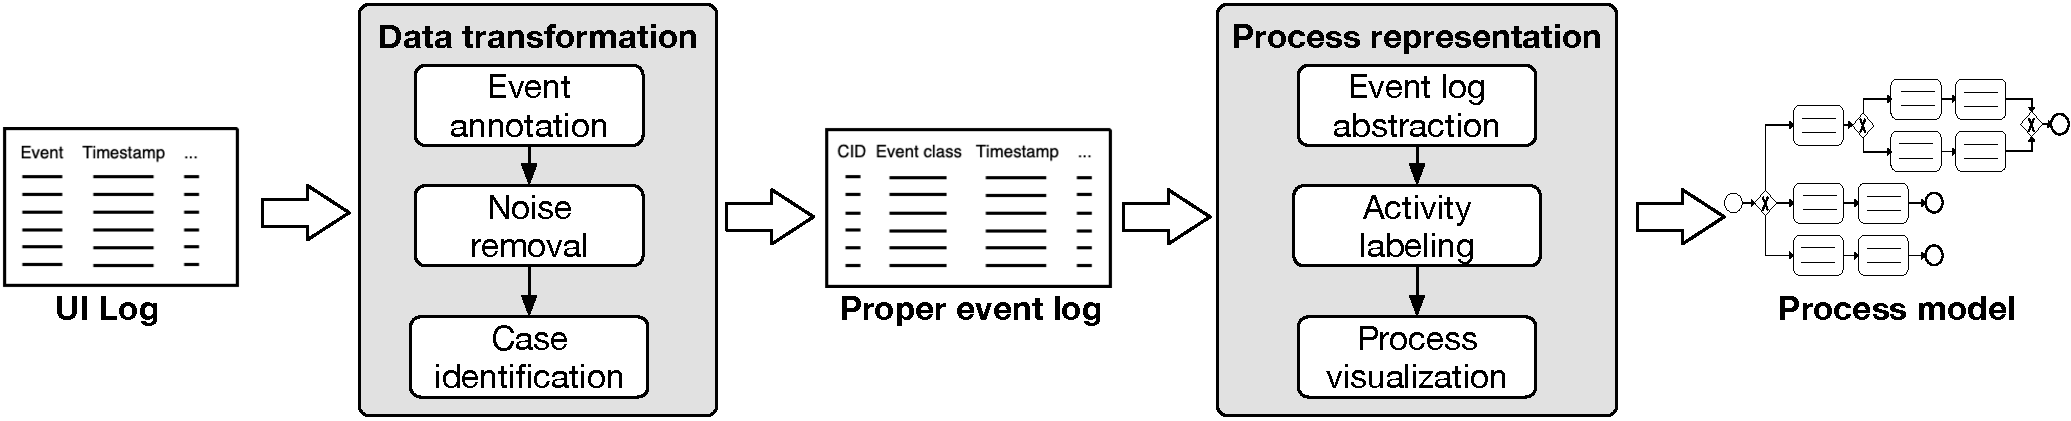
\includegraphics[width=\textwidth]{figures/overview.pdf}
	\caption{Overview of the proposed project}
	\label{fig:approach}
\end{figure}



\subsection{Work programme including proposed research methods}
\label{sec:workprogramme}

\todo{Open questions / points:}
\begin{itemize}
	\item \todo{I feel we need to find a real UI log or we should probably mention that we will create one. Given available software, this is not a big deal, but currently this topic is not covered.}
	\item \todo{We need to streamline the terms: technique, approach, mechanism, component. \textbf{Discussed but need to implement}}
\end{itemize}

\mypar{Package structure} We divided the work programme into two work streams (WS1 and WS2) and a total of six work packages (WP1 to WP6). WS1 will be led by the University of Mannheim and consists of WP1 to WP3. WS2 will be led by the Kühne Logistics University and consists of WP4 to WP6. We have designed the two work streams in such a way that they can be executed independently from each other. We achieved this by making sure that WP4 can build on publicly available, traditional event logs until the first results from WP3 are available. Therefore, both work streams can start in parallel. 

\mypar{Research method} We will achieve our objectives through the design, implementation, and evaluation of novel process mining approaches. The implementation of the proposed approaches will be conducted in Python, based on the \textit{PM4Py} process mining framework\footnote{\url{https://pm4py.fit.fraunhofer.de/}}. The evaluation will be primarily based on publicly available real-world event logs\footnote{\url{https://www.tf-pm.org/resources/logs}}, whereas WP6 will focus on empirical usefulness trough user experiments. By manually creating gold standards for our evaluation data sets, we will test the techniques developed in each WP with respect the specific WP objective. We will use the evaluation results both during the project for improving our techniques and at the end of the project in the context of a summative evaluation at the end of WP6. \todo{Add note about widely available tools and the opportunity to obtain additional if we desire.}

\subsubsection{Work package 1: UI log enrichment (X PM)}
\label{sec:wp1}

We have already shown that UI logs contain a number of relevant attributes for each event. While these attributes may substantially differ per event in a real-world UI log, there is one attribute that is always missing in UI logs in comparison to traditional event logs: an event label revealing what precisely happened. To illustrate this, consider the shortened version of our UI log in \autoref{fig:example_short}. In a traditional event log, event 1 would probably carry a label such as ``\textit{Receive order}''. In the present UI log, we see that the event was a ``\textit{click}'' on a ``\textit{list}'' in the application ``\textit{Outlook}''. That this click relates to receiving an order from a customer can only be inferred from the associated e-mail. Events 4 and 14 also highlight the importance of proper event labels for classifying events. Looking at the key attributes \textit{Event}, \textit{Application}, \textit{Element label}, and \textit{Element type}, they seem to be identical. However, in fact, event 4 leads the user to a log in screen (the password entry succeeds the event), while event 14 completes the log in process (the password entry precedes the event). Proper labels could have clarified this difference. Here, only the \textit{URL} attribute helps to recognize that the specific application context differs. Unfortunately, the application in which an event occurred is sometimes hard to determine. For example, consider events 4, 7, and 13. According to the UI log, these events all occurred in the context of the application ``\textit{Chrome}'', i.e., an Internet browser. However, a brief analysis of the respective URL attributes reveals that event 4 relates to Salesforce and event 13 relates to Facebook. The fact that also event 7 relates to Salesforce is actually hard to identify since the URL structure of Salesforce changes once the user has logged into the application. Given that we intend to build on the semantics of the UI log events, we need to respectively enrich the raw event data from the UI log such that it is clear \textit{what} happened and \textit{where}. 

\begin{figure}[h!]
	\centering
	\begin{adjustbox}{max width=\textwidth}
		\begin{tabular}{llllllll}
			\hline\noalign{\smallskip}\noalign{\smallskip}
			\textbf{ID} &\textbf{Timestamp}&\textbf{Event}&\textbf{Application}&\textbf{Element label}&\textbf{Element type}&\textbf{Element value}&\textbf{URL}\\
			\noalign{\smallskip}\hline\noalign{\smallskip}
			1&08:35.2&click&Outlook&Customer X - O123&list&Please initiate an order …&-\\\noalign{\smallskip}
			...&...&...&...&...&...&...&...\\
			4&08:39.7&click&Chrome&Log in&button&-&https://www.salesforce.com/\\\noalign{\smallskip}
			5&08:40.0&change&Chrome&Password&text field&-&https://login.salesforce.com/\\\noalign{\smallskip}
			6&08:40.5&click&Chrome&Submit&button&-&https://login.salesforce.com/\\\noalign{\smallskip}
			7&08:52.6&click&Chrome&New Account&button&-&https://com.lightning.force.com/home\\\noalign{\smallskip}
			...&...&...&...&...&...&...&...\\
			13&08:40.0&change&Chrome&Password&text field&-&https://www.facebook.com/\\\noalign{\smallskip}
			14&08:42.9&click&Chrome&Log in&button&-&https://www.facebook.com/\\\noalign{\smallskip}
			15&08:42.9&click&Chrome&Messenger&button&-&https://www.facebook.com/\\\noalign{\smallskip}
			...&...&...&...&...&...&...&...\\
			\hline\noalign{\smallskip}
		\end{tabular}
	\end{adjustbox}
	\caption{Shortend version of UI log from \autoref{fig:example}}
	\label{fig:example_short}
\end{figure}

\mypar{Semantic annotation - What} Available process analytics techniques leveraging semantics (e.g., \cite{leopold2012probabilistic,leopold2015_jss,van2021natural}) typically expect that each event can be associated with at least one \textit{action} and at least one \textit{business object}. Building on the example introduced above, the action for event 1 is ``\textit{receive}'' and the business object is ``\textit{order}''. While there are several techniques to derive actions and business objects from labels \cite{leopold2012refactoring,leopold2019using,rebmann2021extracting}, we need to infer these components from the available UI attributes. Therefore, we will develop a process-specific feature extraction technique, which identifies those textual attributes that have the specific roles of actions and business objects. To achieve this, we will combine and adapt existing techniques for the recognition of semantic process components in textual attributes~\cite{rebmann2021extracting} and the extraction of actions from free-text log attributes~\cite{gupta2020analyzing}. Specifically, we will first use graph-based topic discovery algorithms, such as CorePhrase \cite{hammouda2005corephrase}, to detect which attributes carry relevant information. Then, we will use a tagging mechanism based on BERT \cite{Devlin2019} to identify relevant actions and business objects. 

\mypar{Semantic annotation - Where} In traditional event logs, the application in which an event occurred is typically clear. That is, because the application itself records the occurrence of the event. In UI logs, the recording of the event is conducted independently of the used application(s). While the active application is captured in the \textit{application attribute} of the UI log, more and more business applications are browser-based (e.g. Salesforce, Office 365, Basecamp). Hence, the specific \textit{sub application} of many events must be inferred from the associated URL. To achieve this, we mainly build on string matching techniques. First, we check whether the application from the \textit{application attribute} is an Internet browser. This is accomplished by consulting Wikipedia via the MediaWiki Action API\footnote{\url{https://www.mediawiki.org/wiki/API:Main_page}}. Second, in case the application is an Internet browser, we resolve the URL via string matching. To illustrate this, consider event 4 from \autoref{fig:example}. After removing URL-specific prefixes and suffixes, we obtain ``\textit{salesforce}'', which can be easily verified as a business application using Wikipedia. For events where this strategy does not deliver a conclusive result, we look at the event context. For example, for event 7, the string matching strategy is unlikely to deduce that this event occurred in Salesforce. However, when looking at log context, we can clearly identify a number of sub applications, such as Salesforce (from event 4) and Facebook (from event 13). Although the URL of event 7 is rather cryptic, a string matching against these two available options, would clearly identify Salesforce as the most likely sub application. In this way, we resolve URLs and enrich the UI log with the specific sub application in which each event occurred.  

\mypar{Outcome} The outcome of this work package is a technique the enriches the original UI log with three new attributes: \textit{action}, \textit{business object}, and \textit{sub application}. These additional attributes serve as an important basis for the semantic analyses in the subsequent work packages.  


\subsubsection{Work package 2:  Noise removal (X PM)}
\label{sec:wp2}

UI logs often contain events that do not relate to the business process under investigation, such as events related to private activities (e.g., checking Facebook) or to non-related business activities (e.g., filing a reimbursement form of a business trip).
Given that process mining techniques assume that the events in a log relate to a single process, these irrelevant events, also referred to as \emph{noise}, need to be identified and removed from a UI log.

While various noise detection techniques already exist (cf., \autoref{sec:stateoftheart}), these  inherently approach noise detection from a different angle. Particularly, they aim to detect process behavior that stands out in terms of frequency (such as rare occurrence of an order being accepted before it is created), i.e., they try to \emph{detect events that are behavioral anomalies}, e.g., caused by recording errors.
Instead, when dealing with UI logs, we need to \emph{detect events that do not relate to the process at hand}. 

\mypar{Semantic noise detection}
Therefore, to approach this task, we propose to develop a semantic noise detection approach tailored to the specifics of UI logs, which aims to classify events as \emph{process relevant} or not. 
To achieve this, we transform the textual attribute values associated with each event into a feature vector, after applying standard preprocessing steps such as lemmatization and stop-word removal. In this manner, we encode both general event information in features, as well as process-specific information extracted in the previous step, i.e., the event's action, business object, and system.

Once events are transformed in such feature vectors, noise identification can be approached as either a single-class or a two-class classification problem, using state-of-the-art text classifiers, such as a fine-tuned BERT~\cite{Devlin2019} model. The former involves training a classifier that recognizes which events are related to a specific process, e.g., by assuming that the majority of events in a UI log are related to that. While such an approach thus would not require any user input, the classification accuracy may be improved in a two-class setting, where users explicitly label some events as process relevant and irrelevant, so that few-shot learning techniques can be employed~\cite{yu2018diverse}.

Although such classifiers can be employed with just a UI log as input, we will also incorporate mechanisms that allow user to provide additional domain-specific information about the process at hand, such as textual documentation or (high-level) process models, which can help the classifier to better distinguish process relevant from irrelevant events.

\mypar{Outcome}
The outcome of this work package is a classification approach that identifies irrelevant events in a UI log. The approach will be applicable without requiring any additional user input, though users may improve the approach's accuracy through manual labeling of events, as well as by supplying further process-specific artifacts (e.g., a process model) as input.
%This work package focuses on the classification of events in a UI log and the subsequent identification and  removal of irrelevant, i.e., noisy, ones.
%
%\mypar{Event classification}
%\todo{maybe this should be a separate work package? since it also comes with some particular challenges}
%Process mining techniques assume that each event in a log is associated with a particular event class, denoting the action to which the event corresponds~\cite{van2016data}, such as ``\emph{accept order}'' or ``\emph{pay invoice amount}''.
%However, such event classes are not readily available for UI logs. Rather, as shown in  \autoref{fig:example}, events are characterized by various attributes in their payload, which jointly indicate the type of step that is being performed. 
%%For instance, in the form of  the respective application (e.g., Outlook or Chrome) and other details, such as the specific element in the application (e.g., an e-mail or a particular window) and relevant values (e.g., the subject and content of an e-mail). 
%To transform a UI log into an event log that can be employed in process mining, 
%each event needs to be assigned a specific event class based on its payload attributes, which may differ across UI logs or even for different events in the same log. For example, we strive to recognize that certain e-mails refer to the \emph{creation of an order}, whereas other e-mails may correspond to the \emph{handling of an order}. Though these are  two distinct process steps, they nonetheless involve the same application (e.g., Outlook), element (a particular e-mail), and likely the same e-mail subject. Therefore, we need to recognize that the content of the e-mail, as well as its position in a log, relative to related events, determine the event class in this case.
%
%To perform this classification, we recognize that process steps  can be primarily characterized by a combination of a business object (e.g., an \emph{order} or a \emph{ticket}) and an action applied to the object (e.g., \emph{create} or \emph{handle})~\cite{ref}. 
%To recognize these two components in UI events, we aim to combine and adapt existing techniques for the recognition of semantic process components in textual attributes~\cite{rebmann} and the extraction of actions from free-text log attributes~\cite{gupta2020analyzing}. Afterwards the identified event classes can be refined or grouped by employing techniques for the recognition of duplicate~\cite{ref} or polluted event labels~\cite{ref}.
%
% 
% 
% \mypar{Noise removal}
%
%\begin{itemize}
%\item Would be great to go beyond rules here. 
%\item Type 1: Repetitive actions, actions without any effect, and actions that overwrite past actions. 
%\item Type 2: Non-business related stuff: Facebook etc. However, also irrelevant e-mails.
%\item Can we use some sort of semantic angle here? Not sure whether we can determine the domain of a process and just kill anything that is unrelated or so. 
%\end{itemize}
%
%\mypar{Outcome}

\subsubsection{Work package 3: Case identification (X PM)}
\label{sec:wp3}

Once the irrelevant events have been filtered out of a UI log, we next need to recognize which events belong to the same process instance, e.g., to the same customer order or service ticket, a task referred to as \emph{case identification}.

Existing techniques that address this task in general process mining settings primarily base the identification on co-occurrence statistics, which reveal behavioral regulations in an event log (cf., \autoref{sec:stateoftheart}). While such techniques work well for relatively structured settings, their performance deteriorates for event logs stemming from more flexible environments in which the execution of several cases overlaps, such as e.g., seen in the example of \autoref{fig:example}, the first three events each start a new process instance, by initiating three different orders in a batch-like manner.

\mypar{Instance-based event matching}
Recognizing this challenge, this work package sets out to develop a new approach for case identification, tailored to the specifics of UI logs, by building on semantic matching technology.
Specifically, to determine the likelihood that events belong to the same case from a semantic viewpoint, e.g., because both refer to a same order ID or mention the same customer name, we frame the comparison of the events as an \emph{instance-based schema matching} task. For this, we recognize that events stemming from a particular application can be represented as instance in a particular schema (characterized by their payload attributes), enabling the application of existing matching techniques (cf., \cite{somerefs}).

\mypar{Optimization} Having obtained similarity scores between individual events, these scores can then be used together with behavioral regularities identified by existing techniques~\cite{ref}, and cardinality constraints (e.g., each event belongs to exactly or at most one case), to establish an optimization problem, specifically using Markov logic formulation. By solving this problem, we will obtain an event grouping that maximizes the semantic similarity and respects the identified behavioral regularities.

\mypar{Outcome}
The outcome of this work package is a case identification approach that assign case identifiers to the events in a (filtered) UI log, such that the new log encompasses a number of cases, each corresponding to a sequence of events related to the same process instance.


\subsubsection{Work package 4: Log abstraction (X PM)}
\label{sec:wp4}

Even after transformation into a proper event log, the logs stemming from UI recordings comprise low-level event data, in which each event corresponds to a small action performed by a user. This fine-granular nature makes the data unsuitable for meaningful process analysis. This particularly holds for process discovery, since the application of discovery techniques on low-level event logs yields so-called \emph{spaghetti models}, as e.g., depicted in \autoref{fig:spaghetti}.

\begin{wrapfigure}{r}{0.5\textwidth} 
	\vspace{-20pt}
	\begin{center}
		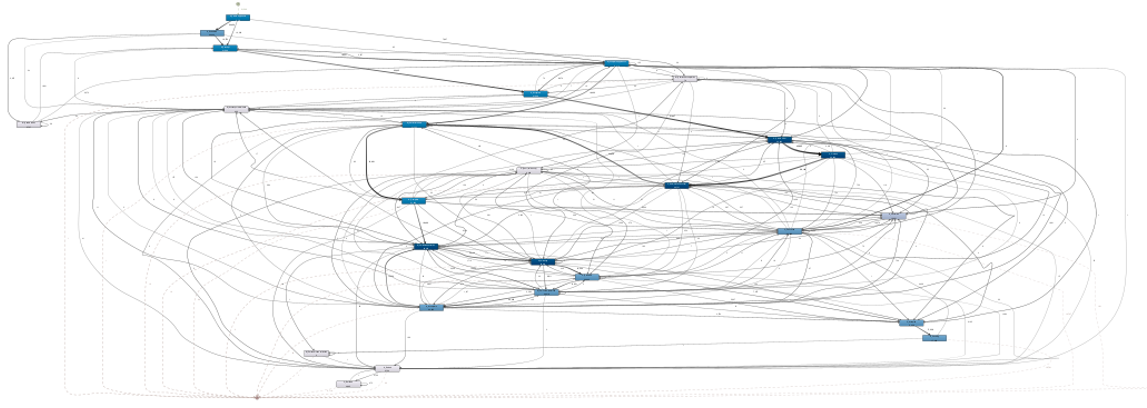
\includegraphics[width=\linewidth]{figures/spaghettiprocess.png}
		\caption{A so-called spaghetti process model}
		\label{fig:spaghetti}
	\end{center}
	\vspace{-20pt}
	\vspace{1pt}
\end{wrapfigure} 

To tackle this issue, log abstraction is a commonly used to lift the event sequences of a log to a more abstract representation, by grouping low-level events into high-level activities. 
As discussed in \autoref{sec:stateoftheart}, various techniques for this purpose exist. Yet, their focus is on \emph{how} the abstraction is conducted, rather than \emph{what properties} the abstracted log shall satisfy. Without dedicated control on the result of log abstraction, however, it is hard to ensure that an abstraction is appropriate for a particular context or specific analysis goal.
This is particularly problematic in the context of UI logs, since these have clear characteristics that should guide the log-abstraction task.

\mypar{Constraint-driven log abstraction}
To overcome this limitation, we propose to develop an approach for \emph{constraint-driven log abstraction}, which it supports a declarative characterization of the properties the abstracted log shall adhere to, in order to be meaningful for downstream analysis. While our approach shall support a broad range of constraint types, common ones to impose in the context of UI logs are for instance constraints that ensure that each high-level activity only comprises events that stem from the same application (to ensure semantic cohesion) or occurred within a certain timespan of each other (to ensure behavioral cohesion). 

Given such a set of user-defined constraints, our approach will aim to identify an optimal log abstraction, which groups together low-level event classes into high-level activities, such that a certain distance function, quantifying the behavioral and semantic similarity of events in an activity, is maximized, while still meeting the imposed constraints.

\mypar{Solution algorithms}
To guarantee an optimal solution, we will initially develop an approach for exhaustive log abstraction. Yet, striving for more efficient processing, we will also provide a heuristic version that is guided by behavioral dependencies found in the log, e.g., by recognizing certain event classes that shall never be grouped into a single activity, due to their relative positions in traces.
As such, this heuristic version shall aim to considerably improve the computation time, with limited impact on the quality of the obtained results.

\mypar{Outcome} The outcome of this work package is an approach that allows users to abstract a low-level event log into high-level activities based on user-defined abstraction requirements. 


\subsubsection{Work package 5: Activity labeling (X PM)}
\label{sec:wp5}

The value of a discovered process model highly depends on the quality of the event labels in the underlying event log. That is, because the event labels are included in the discovered model and, hence, form the basis for what a human can understand about the process \cite{mendling2010activity,Leopold2013Book}. In the context of process modeling, the importance of clear and informative labels has led to a large body of literature concerned with labeling guidelines \cite{mendling2010seven,leopold2015learning} and their automatic enforcement \cite{leopold2013detection,becker2009towards}. The bottom line is that process model activity labels should contain an action provided as an imperative verb (e.g. ``\textit{create}" or ``\textit{send}'') and at least one business object provided as a noun (e.g. ``\textit{order}'' or ``\textit{e-mail}''). Additional information can be provided at the end of the label if required. Examples of proper labels following these rules are ``\textit{Create order}'' or ``\textit{Send e-mail to customer}''. The challenge in the context of this work package is to automatically generate such meaningful labels from for each group of UI events that has been created in the previous work package. To illustrate this, consider the events 4, 5, and 6 from the UI log in Figure \ref{fig:example}. A possible proper label capturing the semantics of these three UI events could be ``\textit{Log into Salesforce}". Automatically generating such a \textit{higher-level label}, however, is highly complex since it requires to infer an overarching activity from the action, business object, and (sub) application attributes.

\mypar{Linguistic relation detection} To generate higher-level labels, we combine the behavioral and the semantic perspective of the process execution. The general observation is that there are different strategies to infer higher-level labels depending on the nature of the considered events. Building on the observations from early work on process model name generation \cite{leopold2014simplifying}, we distinguish three specific strategies: 1) outcome-oriented labeling, 2) decision-based labeling, and 3) holonym-based labeling. The \textit{outcome-oriented labeling} strategy can be applied if the considered set of UI events has a clear result that can be used to described the previous steps. As an example, again consider events 4, 5, and 6 from \autoref{fig:example}. While these three events relate to different specific activities, they can be perfectly summarized by referring to event 4 only, i.e., ``\textit{Log into Salesforce}". The \textit{decision-based labeling} strategy builds on the fact that many processes require the user to make decisions such as rejecting or accepting an offer from a customer. If a considered group of events contains an action that can be related to a decision, this decision will be also used to label the event, even if making the decision is associated with a number of additional events. A possible label for the above-introduced example could be ``\textit{Decide about customer offer}''. The \textit{holonym-based labeling} strategy considers a situation where all (or most) events of the considered event group jointly contribute to a higher-level event. In linguistics, a \textit{holonym} is a term that has a part-of relation with a number of \textit{meronyms}. For example, a ``\textit{finger}'' is a meronym of the holonym ``\textit{hand}''. In the context of the holonym-based labeling strategy, we extend the notion of holonymy to events. This means that the attribute values of action, business object, and (sub) application of events are considered meronyms and we aim to detect the holonym describing the higher-level event. As an example, consider events 11, 12, and 13 from \autoref{fig:example}. While these events are essentially copy and paste operations, they all contribute to a higher-level event that could be described as ``\textit{Create customer account in Salesforce}''. Existing work in the area of process analytics has tried to address the problem of holonymy detection by building on the taxonomy WordNet \cite{leopold2014simplifying}. While WordNet is useful to detect general-purpose holonymy relations (such as the one between ``\textit{finger}'' and ``\textit{hand}''), it does not help to detect more complex and domain-specific relations. Therefore, we will leverage techniques from ontology learning \cite{al2020automatic,wong2012ontology} to automatically derive holonymy relations from general and domain-specific text corpora.    

\mypar{Outcome} The outcome of this work package is a technique that creates an event log with properly labeled higher-level events, i.e., labels consisting at least of an action and a business object. This event log serves as input for the technique from work package 6. 

\subsubsection{Work package 6: Visualization (X PM)}
\label{sec:wp6}

The final step is concerned with the visualization of the process captured in the UI log. In traditional process discovery, this is achieved by generating respective process models. Depending on the employed discovery algorithm, the resulting process model is a simple directly-follows graph \cite{van2019practitioner}, a Petri net \cite{van2004workflow}, a BPMN model \cite{conforti2016bpmn}, or a process tree \cite{leemans2013discovering}. While each algorithm and output representation come with advantages and disadvantages, there is no specific discovery technique available for the UI log generated in WP1 to WP5. The specific challenge is that the original level of granularity of the UI log is not appropriate for visualization since the number of events is too high. Yet, the user might be interested in getting insights into this level to fully understand how the process is executed. What is required is a discovery algorithm that allows the user to adapt the process visualization in a flexible manner with respect to 1) the abstraction level and 2) the general scope. In the context of data warehousing and OLAP \cite{chaudhuri1997overview}, the former corresponds to \textit{drilling down} and \textit{rolling up}, while the latter corresponds to \textit{slicing}. 

\mypar{Slider-based abstraction} The general idea of adapting the level of abstraction using a slider approach is not new and present in many commercial process mining tools such as Celonis\footnote{\url{www.celonis.com}} or Disco\footnote{\url{https://fluxicon.com/disco/}}. However, they implement abstraction by removing arcs or nodes based on their frequency. Our idea is to merge events based on the abstraction mechanism introduced in WP4 and use the approach from WP5 to present meaningful labels to the user. In case the user is interested in more details, the user can drill down on individual events or groups thereof and explore the process on several levels at the same time. To this end, we will build on the ideas on multi-level discovery from \cite{leemans2020using} and adapt them to the specific scenario of slider-based abstraction. 

\mypar{Semantic scoping} Besides adapting the level of abstraction, the user might also want to modify the general scope of the discovered model. It is well imaginable that, for instance, there are specific applications or business objects in the process the user wishes to investigate further or, in the opposite case, remove them from the visualization. We, therefore, introduce a scoping  mechanism that allows the user to select applications and business objects that should be included or removed. We then leverage semantic technology to determine which events should be included or removed from the presented model. Note that this is not trivial since the links between applications and business objects are complex and simply removing all events that do not mention the selected term ``\textit{invoice}'' is certainly to simplistic. Hence, we determine which other events are semantically related to selected business object(s) and respectively include them.    

\mypar{User evaluation} The two mechanisms introduced above are novel and require interaction with users. We, therefore, plan to complement the technical evaluation of our discovery technique with a user study. Specifically, we aim to investigate the effectiveness (in terms of the ability of obtaining insights) and efficiency (in terms of how fast user can obtain insights).      

\mypar{Outcome} The outcome of this work package is a novel discovery technique that can visualize UI logs in a flexible fashion. As such, it completes our overall approach for semantic discovery from UI logs we develop in this proposal. 

%slider idea , visualization: taillired to abstaction approach by using slider approach ; semantic sliding appriach: application or business object "i want more detail on the events with this particular action or business object" 
% semantic sliding abstraction 
% thinkg of variants and implications on that matter 
% results need to be visaluzed somehow; maybe we want to drill down; maybe test with some people? do we need different views? multi-level discovery --> check paper


\subsubsection{Overview on the work plan}

\begin{figure}[bt]
	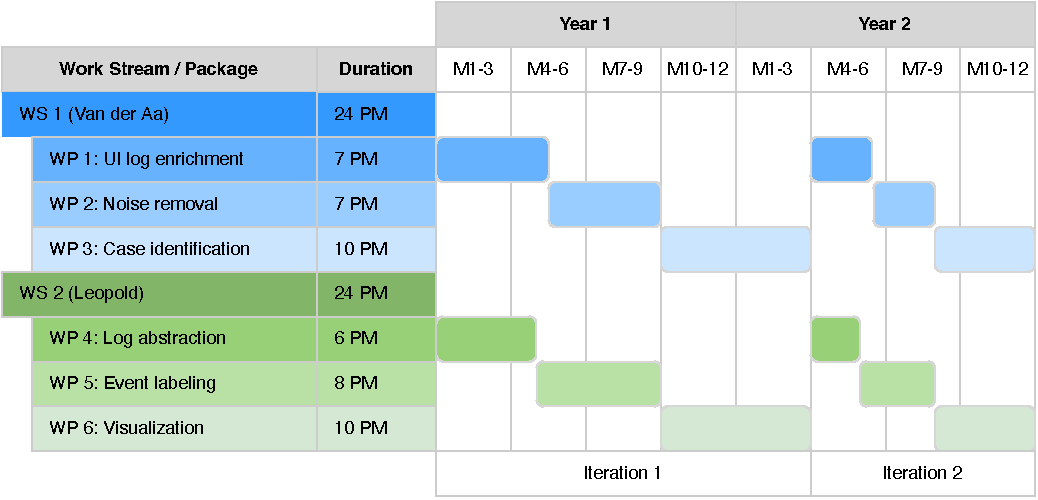
\includegraphics[width=\textwidth]{Figures/Gantt.pdf}
	\caption{Work plan}
	\label{fig:workplan}
\end{figure}

As explained above, the project consists of two work streams and six work packages. Naturally, there are interdependencies among these work packages. Figure \ref{fig:workplan} shows a simplified work plan that mostly abstracts from parallel and overlapping work within each work stream. It is important to highlight that the transitions between two packages will not be as strict as depicted. We are aware of the various interdependencies and will take them into account appropriately.  
There are, for instance, interdependencies between WP1 and WP1. Without an enriched UI log, the noise removal technique cannot build on the newly introduce attributes. This, however, can be addressed by taking the manually created gold standard for the evaluation of WP1 as input for WP2. In this way, the noise removal technique cannot already be developed without needing a ``perfect'' solution for WP1. The rather abstract view on the work plan shown in Figure \ref{fig:workplan} highlights our general idea of having two main iterations:
\begin{itemize}
	\item The first iteration ends after 21 month. At the end of this iteration, there will be a first implemented prototype available. The individual techniques have been evaluated both independently and as a whole. The main outcome from this iteration, therefore, are insights into the strengths and weaknesses of our techniques, which allows us to determine the required improvements and adaptations for the second iteration. 
	\item The second iteration is slightly shorter and will be mainly used to address identified weaknesses and improve the performance of the technique.
\end{itemize} 

Note that these two iterations also help us to account for the interdependencies between the two work streams (as discussed earlier). In the first iteration, WS 2 will build on traditional, freely available event logs, while in the second iteration WS 2 can build on a UI log that has been processed with the techniques from WS1. 



%Note that the work plan shown above allocates a total of 42 project months to 3 years. As explained in Section \ref{sec:staff}, we intend to hire a PhD student for 3 years, which means that remaining 6 project months will be covered by the respective principal investigator of this project. 